% $Header$

\documentclass{beamer}

\setbeamertemplate{bibliography item}[text]

\newcommand\leftidx[3]{%
  {\vphantom{#2}}#1#2#3%
}

\usepackage{eso-pic}
\usepackage{multimedia}
\usepackage[english]{babel}
%\usepackage[pdftex]{graphicx}
\usepackage{algorithm}
%\usepackage[noend]{algorithmic}
%\usepackage[flalign]{amsmath}
%\usepackage{amsmath}
%\usepackage{gensymb}
\usepackage{ftnxtra}
\usepackage{fnpos}

\usepackage{amssymb}
\usepackage{array}
\usepackage{bm}
%\usepackage{amsmath}
\usepackage{placeins}
%\usepackage[noend]{algpseudocode}
\usepackage{wrapfig}
\usepackage{graphicx}
\usepackage{paralist} 
\usepackage{amsfonts}
\usepackage{amssymb}
\def\wl{\par \vspace{\baselineskip}}
\usepackage{graphicx}
\usepackage{array}
\usepackage{booktabs}
\usepackage{tabularx}
\usepackage{siunitx}
\usepackage{caption}


%\makeatletter
%  \renewcommand*\env@matrix[1][c]{\hskip -\arraycolsep
%  \let\@ifnextchar\new@ifnextchar
%  \array{*\c@MaxMatrixCols #1}}
%\makeatother

\DeclareCaptionType{mycapequ}[][List of equations]
\captionsetup[mycapequ]{labelformat=empty}


\def\hlinewd#1{%
\noalign{\ifnum0=`}\fi\hrule \@height #1 %
\futurelet\reserved@a\@xhline}
\usepackage{cite}
\usepackage[normalem]{ulem}
\usepackage{tabu}
\usepackage{mathrsfs}
\usepackage{epstopdf}

\usepackage{subfigure}



%\newcommand\leftidx[3]{%
%  {\vphantom{#2}}#1#2#3%
%}



\usepackage{float}
\usepackage{multirow}
%\usepackage{SIunits}
\usepackage{anyfontsize}
\usepackage{xspace}
\usepackage{dsfont}
\usepackage{subfigure}
%\usepackage{mathrsfs}
\usepackage{bm}
\usepackage{color}
%\usepackage{matlab-prettifier}
%\usepackage{ftnxtra}
%\usepackage{fnpos}
%\makeatletter
%\renewcommand*\env@matrix[1][c]{\hskip -\arraycolsep
%  \let\@ifnextchar\new@ifnextchar
%  \array{*\c@MaxMatrixCols #1}}
%\makeatother

% For matlab-prettifier
%\lstinputlisting[style=Matlab-editor]{FileLocation.m}
%

\usepackage{algorithm}
\usepackage[noend]{algorithmic}
\renewcommand{\algorithmicrequire}{\textbf{Input:}}
\renewcommand{\algorithmiccomment}[1]{$\rhd$ #1}
\renewcommand{\algorithmicensure}{\textbf{Output:}}
\newcommand{\ie}{{\it i.e.},\xspace}
\newcommand{\eg}{{\it e.g.},\xspace}
\newcommand{\cf}{{\it c.f.},\xspace}
\newcommand{\el}{{\it et al.},\xspace}
\newcommand{\etc}{\text{etc.}}
\DeclareFontFamily{OT1}{pzc}{}
\DeclareFontShape{OT1}{pzc}{m}{it}%
              {<-> s * [1.200] pzcmi7t}{}
\DeclareMathAlphabet{\mathpzc}{OT1}{pzc}%
                                 {m}{it}

% FOR CONDITIONS AFTER EQUATION
\newenvironment{conditions*}
  {\par\vspace{\abovedisplayskip}\noindent
   \tabularx{\columnwidth}{>{$}l<{$} @{\ : } >{\raggedright\arraybackslash}X}}
  {\endtabularx\par\vspace{\belowdisplayskip}}
%%%

\newcommand{\ud}{\,\mathrm{d}}

%\usepackage{pseudocode}
\usepackage{resizegather}            
\usepackage{mathrsfs}
\usepackage{bm}
\usepackage{setspace}
\usepackage{multicol}
\usepackage{ulem}
\usepackage{hyperref}
\usepackage{amsmath}
\def \marhes{{\sc Marhes~}}
\usepackage{mathtools}
\usepackage{tikz}
\usepackage{wrapfig}
\DeclareMathAlphabet {\mathbfit}{OML}{cmm}{b}{it}

\newcommand\encircle[1]{%
  \tikz[baseline=(X.base)] 
    \node (X) [draw, shape=circle, inner sep=0] {\strut #1};}

\def\deg{\ifmmode^\circ\else$^\circ$\fi}

\makeatletter
\newcommand{\captionabove}[2][]{%
    \vskip-\abovecaptionskip
    \vskip+\belowcaptionskip
    \ifx\@nnil#1\@nnil
        \caption{#2}%
    \else
        \caption[#1]{#2}%
    \fi
    \vskip+\abovecaptionskip
    \vskip-\belowcaptionskip
}

%\usepackage{bibentry}
%%%%%%%%%%%%%%%%%%%%%%%
%%%%%%%%%%%%%%%%%%%%%%%
%%%%%%%%%%%%%%%%%%%%%%%
% This file is a solution template for:

% - Giving a talk on some subject.
% - The talk is between 15min and 45min long.
% - Style is ornate.



% Copyright 2004 by Till Tantau <tantau@users.sourceforge.net>.
%
% In principle, this file can be redistributed and/or modified under
% the terms of the GNU Public License, version 2.
%
% However, this file is supposed to be a template to be modified
% for your own needs. For this reason, if you use this file as a
% template and not specifically distribute it as part of a another
% package/program, I grant the extra permission to freely copy and
% modify this file as you see fit and even to delete this copyright
% notice. 

\newcommand\AtPagemyUpperLeft[1]{\AtPageLowerLeft{%
\put(\LenToUnit{0.01\paperwidth},\LenToUnit{0.85\paperheight}){#1}}}
%\AddToShipoutPictureFG{
%  \AtPagemyUpperLeft{{\includegraphics[width=1.33 cm,keepaspectratio]{./Images/UNM_Logo.jpg}}}
%}%

%\footnote[frame]{A test footnote in the second column}
\mode<presentation>
{
  \usetheme{CambridgeUS}
  % or ...
  \usecolortheme{dolphin}
  \setbeamercovered{transparent}
  % or whatever (possibly just delete it)
}
\setbeamertemplate{bibliography item}{}

%remove line breaks
\setbeamertemplate{bibliography entry title}{}
\setbeamertemplate{bibliography entry location}{}
\setbeamertemplate{bibliography entry note}{}


\useoutertheme[left]{sidebar}
%\setbeamercolor{headline}{rgb}{fg=white,bg=red}
\setbeamertemplate{footline}{}
\usepackage[english]{babel}
% or whatever

\usepackage[latin1]{inputenc}
% or whatever


\usepackage{times}
\usepackage[T1]{fontenc}
% Or whatever. Note that the encoding and the font should match. If T1
% does not look nice, try deleting the line with the fontenc.


\title[Torque Control] % (optional, use only with long paper titles)
{Experiencing Torque Control}

\subtitle
{A Literary Review} % (optional)

\author[Wilhelmi] % (optional, use only with lots of authors)
{C.~Wilhelmi}%\inst{1}} %\and S.~Another\inst{2}}
% - Use the \inst{?} command only if the authors have different
%   affiliation.

\institute[George Mason University] % (optional, but mostly needed)
{
  %\inst{1}%
  George Mason University \\
  Fairfax, VA
  
}  
%  \and
%  \inst{2}%
%  Department of Theoretical Philosophy\\
%  University of Elsewhere}
% - Use the \inst command only if there are several affiliations.
% - Keep it simple, no one is interested in your street address.

\date[ ] % (optional)
{\today}

\subject{Talks}




\begin{document}

\begin{frame}
  \titlepage
\end{frame}

\begin{frame}{Outline}
  \tableofcontents
  % You might wish to add the option [pausesections]
\end{frame}


% Since this a solution template for a generic talk, very little can
% be said about how it should be structured. However, the talk length
% of between 15min and 45min and the theme suggest that you stick to
% the following rules:  

% - Exactly two or three sections (other than the summary).
% - At *most* three subsections per section.
% - Talk about 30s to 2min per frame. So there should be between about
%   15 and 30 frames, all told.

\section[Introduction]{Introduction}


\begin{frame}{Introduction}{Introduction}
\begin{columns}
    \begin{column}{0.47\textwidth}
The idea of Torque Control will be discussed in the following ways:
\begin{itemize}
	\item Definitions
	\item Problems
	\item Techniques  
	\item Interesting Concept
	\item Takeaway Points
\end{itemize}	
    \end{column}
    \begin{column}{0.5\textwidth}
    		\centering
    		ICUB\footnotemark[1]
        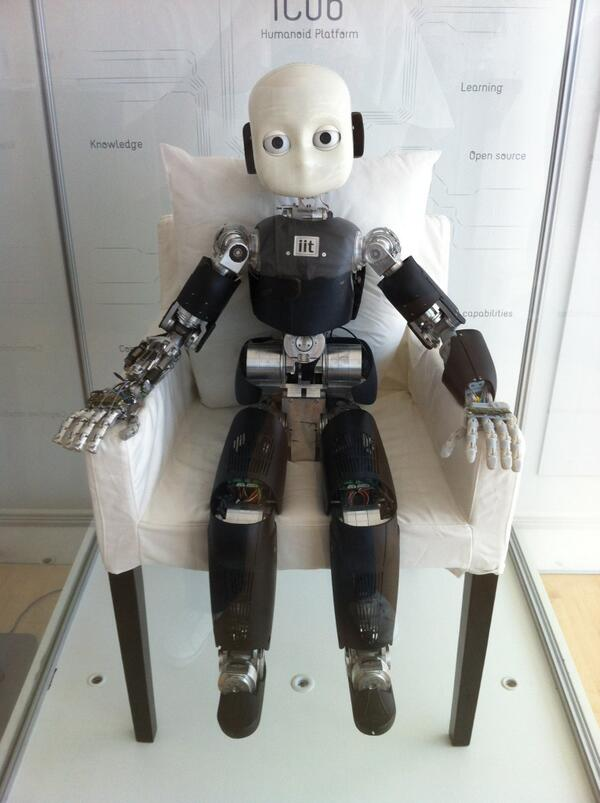
\includegraphics[scale=.15]{./images/creepy_cub.jpg}
    \end{column}
	
	\footnotetext[1]{https://twitter.com/icub}
\end{columns}  

\end{frame}

\section[Definitions]{Important Definitions}
\begin{frame}{Definitions}{Let's All Speak The Same Language}
\begin{itemize}
	\item Asymptotic Stability
	\item Lyapunov Stability
	\item Fuzzy Logic
\end{itemize}
\end{frame}



\section[Problems]{Problems To Deal With}
\begin{frame}
General Issues:
\begin{itemize}
	\item Must manipulate end effector (or end joint) positions to execute a desired command \cite{piltan}
	\item Must minimize or reject disturbances \cite{piltan,6954103}
	\item Conventional controllers need exact dynamical models \cite{piltan}
	\item Extremely nonlinear \cite{SONG2005208,1035149,piltan}
\end{itemize}
PID Controllers\cite{SONG2005208}
\begin{itemize}
	\item Must decouple each joint
	\item Good for slow motion but degradation at faster speeds
\end{itemize}
Torque Controllers:
\begin{itemize}
	\item Excellent control comes at the cost of flux \cite{6954103}
	\item Powerful nonlinear controller that is widely used in robotic manipulators
\end{itemize}
\end{frame}

\section[Techniques]{2011 To Present}
\begin{frame}{Techniques}{Super-Twisting Sliding Mode\cite{6954103}}
%\begin{tabular}{lc}
\begin{columns}
    \begin{column}{0.47\textwidth}
        \begin{itemize}
	\item Fast switching of control inputs
	\item Produces a stable response
	\item The closed loop response is stable if external influences are bounded and gains set to large values
	\item Works well with PWM and inverter switching
	\item STSM control is a second order scheme
	\item Asymptotic convergence
        \end{itemize}
    \end{column}
    \begin{column}{0.5\textwidth}
        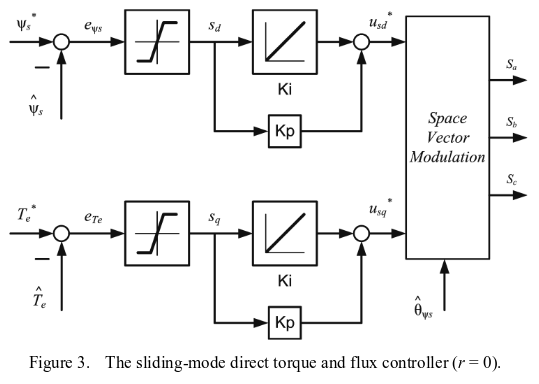
\includegraphics[scale=.25]{./images/direct_torque_flux_controller.png}
    \end{column}
\end{columns}
\end{frame}

\begin{frame}{Techniques}{Super-Twisting Sliding Mode\cite{6954103}}
%\begin{tabular}{lc}
\begin{columns}
    \begin{column}{0.47\textwidth}
        \begin{itemize}
        		\item The nonlinearity of the device can be controlled by changing the exponent $r$ such that $0 \leq r \leq $
			\item Step 1: with $r=0$, select $K_P$ for the desired response time
			\begin{itemize}
				\item the flux rising time has a strong impact on startup peak current
			\end{itemize}
			\item Step 2: with $r=1$, select $K_I$ for the desired overshoot and settling time.  
				\begin{itemize}
					\item Try to not have a visible overshoot and smooth settling
				\end{itemize}
			\item increase $r$ until the torque and flux ripples vanish
        \end{itemize}
    \end{column}
    \begin{column}{0.5\textwidth}
        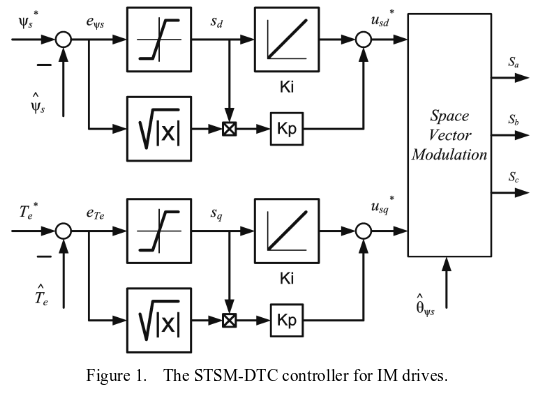
\includegraphics[scale=.25]{./images/stsm_dtc_controller.png}
    \end{column}
\end{columns}
\end{frame}

\begin{frame}{Techniques}{PD Plus Gravity\cite{piltan}}
%\begin{tabular}{lc}
\begin{columns}
    \begin{column}{0.47\textwidth}
        \begin{itemize}
			\item Fuzzy logic parameters can compensate for dynamic parameters
			\item Much simpler to implement than regular torque control problems
			\item Based on Brunousky canonical form
        \end{itemize}
        \begin{align*}
        	\dot{x} &= Ax + Bu \\
        	\dot{x} &= \begin{bmatrix}
        	0 & I \\ 0 & 0
        	\end{bmatrix}x + \begin{bmatrix}
        	0 \\ I
        	\end{bmatrix}N \\
        	N &= B(q)[\dot{q}\dot{q}] + C(q)[\dot{q}]^2 + G(q)
        \end{align*}
    \end{column}
    \begin{column}{0.5\textwidth}
        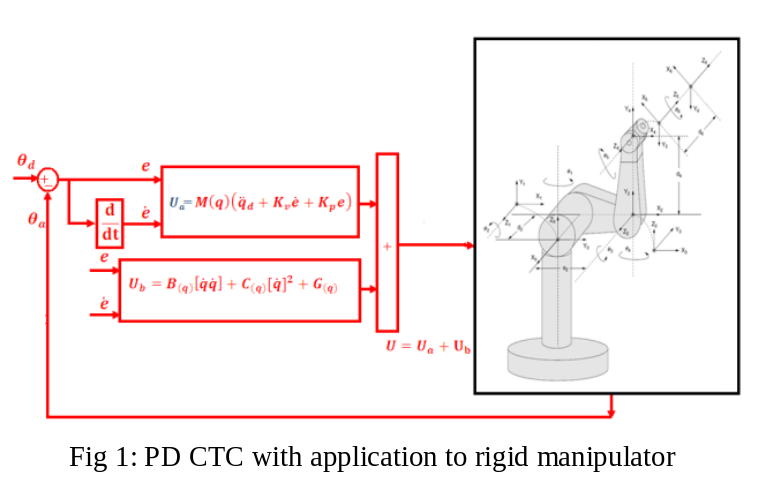
\includegraphics[scale=.2]{./images/pd_ctc_application.png}
    \end{column}
\end{columns}
\end{frame}


\begin{frame}{Techniques}{PD Plus Gravity\cite{piltan}}
%\begin{tabular}{lc}
\begin{columns}
    \begin{column}{0.47\textwidth}
        For the PD Feedback for $N(t)$:
        \begin{equation*}
        \tau = M(q)(\ddot{q}_d + K_D\dot{e} + K_Pe) + N(q,\dot{q})
        \end{equation*}
        When gravity is added into the feedback system:
        \begin{equation*}
        \tau = M(q)(\ddot{q}_d + K_D\dot{e} + K_Pe) + G(q)
        \end{equation*}
        The above has been found to be stable in Lyapunov sense
    \end{column}
    \begin{column}{0.5\textwidth}
        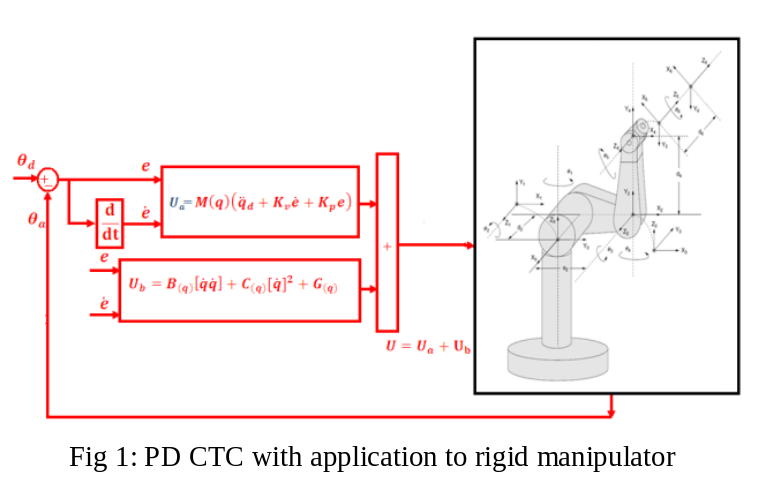
\includegraphics[scale=.2]{./images/pd_ctc_application.png}
    \end{column}
\end{columns}
\end{frame}


\begin{frame}{Techniques}{PD Plus Gravity\cite{piltan}}
%\begin{tabular}{lc}
\begin{columns}
    \begin{column}{0.47\textwidth}
asdf
    \end{column}
    \begin{column}{0.5\textwidth}
        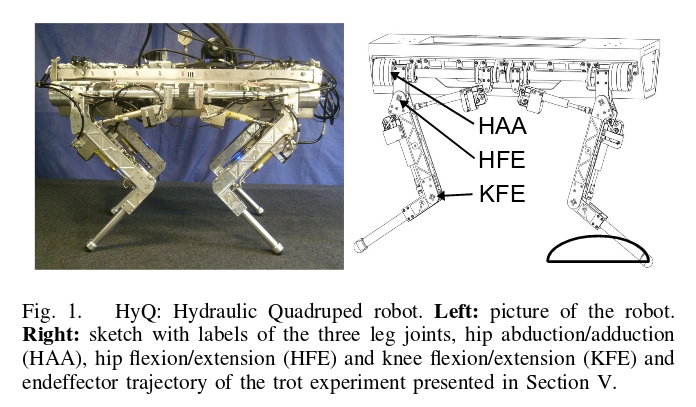
\includegraphics[scale=.2]{./images/quad_robot.png}
    \end{column}
\end{columns}
\end{frame}



\begin{frame}{Techniques}{PD Plus Gravity\cite{piltan}}
%\begin{tabular}{lc}
\begin{columns}
    \begin{column}{0.47\textwidth}
asdf
    \end{column}
    \begin{column}{0.5\textwidth}
        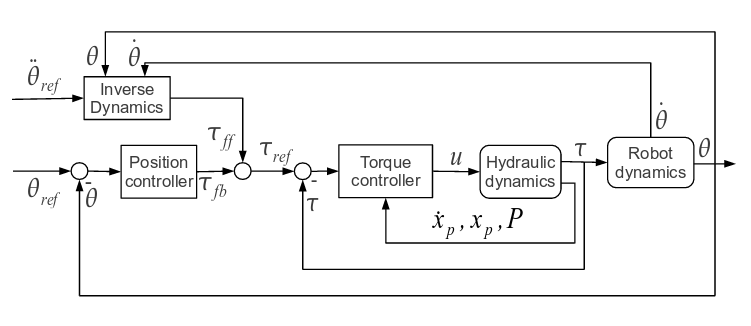
\includegraphics[scale=.2]{./images/dynamics.png}
    \end{column}
\end{columns}
\end{frame}

\section[Conclusion]{Takeaway Points}

\begin{frame}{Takeaway}{What did we learn?}
In conclusion, several items were learned:
\begin{itemize}
	\item Robotic manipulators and joints are highly nonlinear
	\item Torque control has several different ways to solve
	\item Stability criteria can be met
	\item Other methods exist such as phase angle \cite{7525846}
	\item Latex Beamer is just not fun
\end{itemize}
\end{frame}

\begin{frame}[allowframebreaks]
        \frametitle{References}
       % \bibliographystyle{plainnat}
        \bibliographystyle{IEEETran}
        \bibliography{LitReviewBib.bib}
\end{frame}
\end{document}


